%!TEX root =  autocontgrlp.tex
\begin{comment}
\section{Approximate Linear Programming: Successes and Challenges}
When the MDP has a large number of states, it is difficult to solve for $J^*$ using either the linear program \eqref{mdplp} or other full state representation methods such as value iteration or policy iteration \cite{BertB}. A practical solution is to resort to function approximation. Linear function approximation, wherein the solution is searched in the subspace spanned by the column vectors of a given feature matrix $\Phi$.
The approximate linear program (ALP) is obtained by making use of LFA in the LP, i.e., by introducing the new variables $r\in \R^k$ and adding the extra constraint $J=\Phi r$ in \eqref{mdplp} with $\Phi \in \R^{n\times k}$ \citep{SchSei85}.
By substitution, this leads to
\begin{align}\label{alp}
\begin{split}
\min_{r\in \R^k}\, &c^\top \Phi r\,\,\,
\text{s.t.}\mb \Phi r\geq T \Phi r,
\end{split}
\end{align}
where $J\geq TJ$ is a shorthand for the $nd$ constraints in \eqref{mdplp} and $\Phi$ is a feature matrix whose first column is $\one$. Unless specified otherwise we use $\tr$ to denote an arbitrary solution to ALP, and we let $\tj=\Phi \tr$ to denote the corresponding approximate value function and $\tu$ to denote the greedy policy w.r.t. $\tj$.
The following is a preliminary error bound for ALP from \cite{ALP}:
\begin{theorem}[Error Bound for ALP]
\begin{align*}
\norm{J^*-\tj}_{1,c}\leq \frac{2}{1-\alpha}\min_{r}\norm{J^*-\Phi r}_\infty
\end{align*}
\end{theorem}
%For a more detailed treatment of ALP and sophisticated bounds, the reader is referred to \cite{ALP}.
%\subsection{Approximating the Constraints}
The ALP is a linear program in $k$ ($<<n$) variables as opposed to the LP in \eqref{mdplp} which has $n$ variables. Nevertheless, ALP has $nd$ constraints (same as the LP) which is an issue when $n$ is large and calls for constraint approximation/reduction techniques. Most works in literature make use of the underlying structure of the problem to cleverly reduce the number of constraints of ALP. A good example is \cite{gkp}, wherein the structure in factored linear functions is exploited. The use of basis function also helps constraint reduction in \cite{Mor-Kum}. In \cite{ALP-Bor}, the constraints are approximated indirectly by approximating the square of the Lagrange multipliers. In \cite{petrik} the transitional error is reduced ignoring the representational and sampling errors.\par
The most important work in the direction of constraint reduction is constraint sampling \cite{CS} wherein a reduced linear program (RLP) is solved instead of ALP. While the objective of RLP is same as that of ALP, RLP has only $m<<nd$ constraints \emph{sampled} from the original $nd$ constraints of ALP.  The following is a preliminary error bound for RLP from \cite{CS} holds for a special sampling distribution which is dependent on the optimal policy $u^*$ (see \cite{CS} for a detailed presentation):
\begin{theorem}[Error Bound for RLP]
Let $\mu_{u^*}\eqdef(1-\alpha)c^\top (I-\alpha P_{u^*})^{-1}$ be a probability distribution (of discounted number of visits) over the states $S$. Define $\psi_{u^*}$ to be the distribution amongst state-action pairs such that $\psi(s,a)\eqdef \frac{\mu_{u^*}}{d}$ and define $\theta\eqdef=\frac{1+\alpha}{2 c^\top J^*}\underset_{r\in \N}{\sup}\parallelJ^*-\Phi r \parallel_\infty$. Then for a given $\epsilon>0$ and $\delta>0$ it holds that
\begin{align*}
\norm{J^*-\Phi\tilde{r}_{RLP}}_{1,c}\leq \norm{J^*-\Phi\tilde{r}}_{1,c}+\epsilon \norm{J^*}_{1,c}
\end{align*}
for all $m\geq \frac{16d\theta}{(1-\alpha)\epsilon}\big(k\ln\frac{48d\theta}{(1-\alpha)\epsilon}+\ln \frac{2}{\delta}\big)$.
\end{theorem}
%A major gap in the theoretical analysis is that the error bounds are known for only a specific RLP formulated using idealized assumptions, i.e., under knowledge of $u^*$. However, RLP has be found to do well empirically in domains such as Tetris \cite{CST} and controlled queues \cite{CS}.
\subsection{Open Questions}
Interestingly, RLP has nevertheless been found to do well empirically in domain such as Tetris \cite{CST} and controlled queues \cite{CS} even when the constraints were sampled using distribution other than the ideal distribution. This fact indicates a gap in the theoretical analysis and points to the need for a more elaborate theory that addresses the issue of constraint approximation. In this paper, we answer the following questions related to constraint reduction in ALP that have so far remained open. \\
$\bullet$ As a natural generalization of RLP, what happens if we define a generalized reduced linear program (GRLP) whose constraints are positive linear combinations of the original constraints of ALP?\\
$\bullet$ Unlike \cite{CS} which provides error bounds for a specific RLP formulated using an idealized sampling distribution, is it possible to provide error bounds for any GRLP (and hence any RLP)?
In this paper, we address both of the questions above.
\end{comment}
\section{Generalized Reduced Linear Programming}\label{sec:grlp}
The Generalized Reduced Linear Program is given as:
\begin{align}\label{grlp}
\begin{split}
&\underset{r\in \N\subset R^k}{\min}\, \, c^\top \Phi r\,\,\,\,\\
&\text{s.t.}\mb  \,W^\top E\Phi r\geq W^\top H \Phi r,
\end{split}
\end{align}
where we assume that $W \in \R^{nd\times m}_+$ is a matrix with all positive entries which specifies the linear combination of constraints.  We denote an arbitrary solution to GRLP by $\hr$, and the approximate value function by $\hj=\Phi \hr$ and use $\hu$ to denote the greedy policy w.r.t. $\hj$.\\
\textbf{RLP as a special case:} Recovering RLP \eqref{rlp} as a special case of GRLP \eqref{grlp} can be accomplished by setting $W$ to the matrix with the $i^{th}$ column having $1$ corresponding to the constraint that was sampled (implicitly assuming that there is a natural ordering of the $nd$ constraints) and all the other entries as $0$. The $\N$ in RLP \eqref{rlp} is retained in GRLP \eqref{grlp} as well. For $m=nd$ and $W=I_{nd\times nd}$, GRLP is same as ALP.\\
\textbf{Linear function approximation in Primal and Dual Variables:} Let us look at the Lagrangian of ALP and GRLP in
\eqref{lag} and \eqref{lag2} respectively, i.e.,
\begin{align}\label{lag}
\tilde{L}(r,\lambda)=c^\top \Phi r+\lambda^\top (T\Phi r-\Phi r), \\ \label{lag2}\hat{L}(r,q)=c^\top \Phi r+q^\top W^\top (T\Phi r-\Phi r).
\end{align}
Thus, when $Wq = \lambda$, i.e., when $W$ is a set of basis functions that allow
a low dimensional linear representation of the dual variables $\lambda$,
the two problems are the same.
%Note that $ Wq\approx \lambda$ in \eqref{lag2} is linear function approximation of the Lagrange multipliers.
Hence, while ALP employs LFA in its objective function (i.e., use of $\Phi r$), GRLP employs linear approximation both in the objective function ($\Phi r$) as well as the constraints (use of $W$).
%Further, $W$ can be interpreted as the feature matrix that approximates the Lagrange multipliers as $\lambda\approx Wq$, where $\lambda \in \R^{nd}, r\in \R^m$.
To get a sense of how $W$ should be chosen, recall that
the optimal Lagrange multipliers are the discounted number of visits to the ``state-action pairs'' under an optimal policy $u^*$, i.e.,
\begin{align}
\lambda^*(s,u^*(s))&=\big(c^\top(I-\alpha P_{u^*})^{-1}\big)(s)\nn\\
&= \big(c^\top(I+\alpha P_{u^*}+\alpha^2 P_{u^*}^2+\ldots)\big)(s),\nn\\
\lambda^*(s,a)&=0, \qquad \text{for all } a \neq u^*(s),\nn
\end{align}
where $P_{u^*}$ is the probability transition matrix under $u^*$ ($P_{u^*}(s,s') = P_{u^*(s)}(s,s')$, $s,s'\in S$) \cite{dolgov}. Even though we might not have the optimal policy $u^*$ in practice, the fact that $\lambda^*$ is a probability distribution and that it is a linear combination of $\{P_{u^*},P^2_{u^*},\ldots\}$ hints at the kind of features that might be useful for constructing the $W$ matrix.
\FloatBarrier
%\begin{figure}[h!]
\centering
%\resizebox{columnwidth}{2cm}{
\begin{tikzpicture}[domain=-10:7.7,scale=0.6,font=\small,axis/.style={very thick, ->, >=stealth'}]
%\draw[line,thick,->] (-1,-0.625)--(4,-0.625);
%\draw[line,thick,->] (0,-1)--(0,4);
%\draw[line,thick,-](-0.2,-0.6)--(1,3);
\draw[line,thick,-](0.5,3.5)--(1,1);
\draw[line,thick,-](1,1)--(3,1.5);
\draw[line,thick,-](3,1.5)--(4,2.1);
\node[](one) at (2,2.3){\text{$J\geq TJ$}};
\node[rotate=-45](seven) at (-0.5,2.3){\text{\tiny $W^\top J\geq W^\top TJ$}};
\node[](two) at (-0.3,-0.5){\text{$\Phi r$}};
\node[](three) at (0.7,0.7){\text{$J^*$}};
%\draw[line,thick,-](0,0)--(4,2.5);
 \draw [ultra thick, draw=white, fill=gray, opacity=0.5]
       (0.5,3.5)--(1,1)--(3,1.5)--(4,2.1) -- cycle;
\draw[line,thick,-](-1,-0.625)--(3,1.8750);
 \fill (1,1)  circle[radius=2pt];
 \fill (2,1.25)  circle[radius=2pt];
 \fill (0.5,0.3125)  circle[radius=2pt];
\draw[line,dashed,-](-1,0.1)--(6,1);
\draw[line,dashed,-](-1,0.1)--(-2,5);
 \draw [ultra thick, draw=white, fill=gray, opacity=0.2]
       (-1,0.1)--(6,1)--(-2,5) -- cycle;
\node[] (four) at (2,0.8){\text{$\tilde{J}_c$}};
\node[] (six) at (0.5,-0.1){\text{$\hat{J}_c$}};
\end{tikzpicture}
%}
\caption{The outer lightly shaded region corresponds to GRLP constraints and the inner dark shaded region corresponds to the original constraints. The main contribution of the paper is to bound $||J^*-\hat{J}_c||$.}
\label{cartoon}
\end{figure}


\begin{figure}
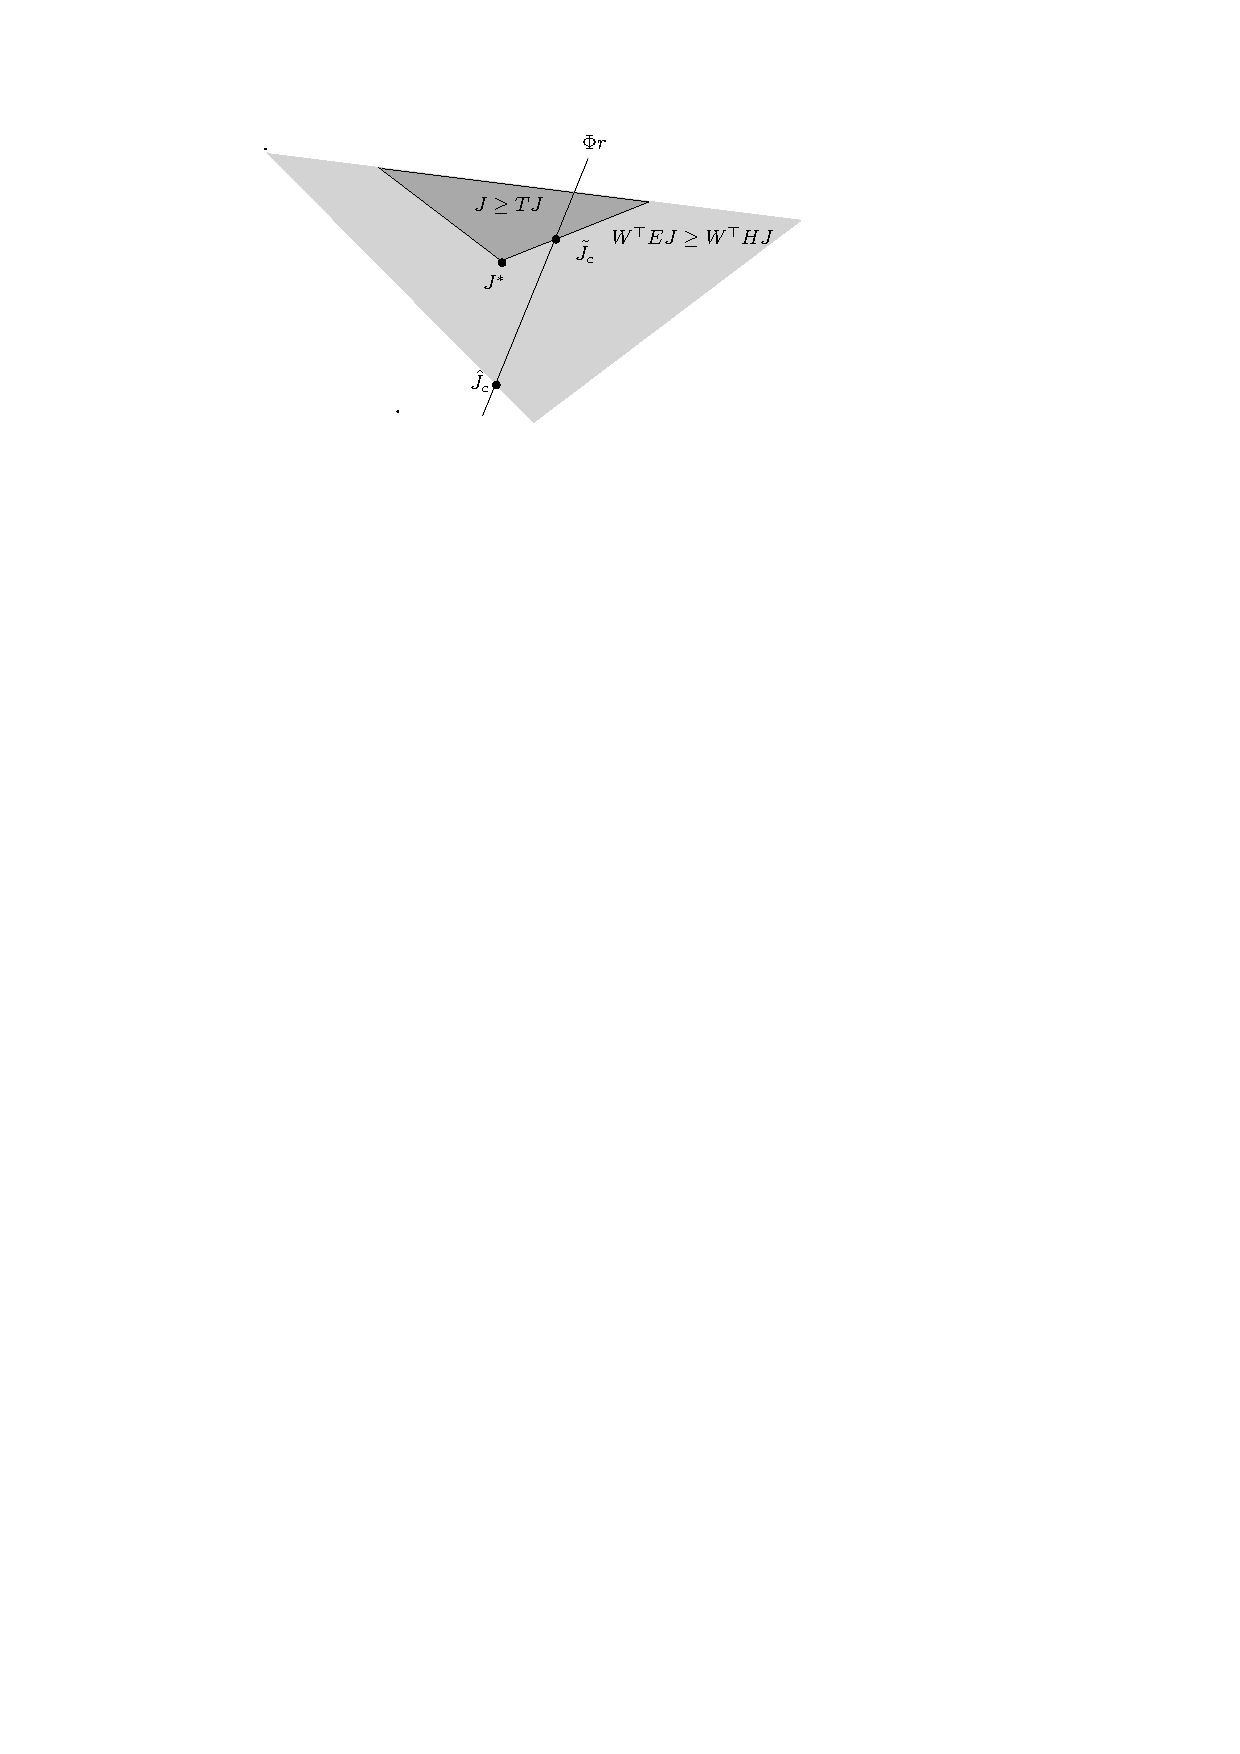
\includegraphics[scale=0.7]{cartoon_grlp.pdf}
\caption{
%\normalsize
The outer lightly shaded region corresponds to GRLP constraints and the inner dark shaded region corresponds to the original constraints. The main contribution of the paper is to bound $\norm{J^*-\hat{J}_c}$.}
\label{cartoon}
\end{figure}
\Cref{cartoon} shows the solutions to the LP, ALP and GRLP respectively. The error in ALP solution has already been studied in \cite{ALP}. Our objective is to study the extra source of error due to constraint approximation.
\section{Main Results}
In this section we present the main results of this paper in \Cref{cmt2} (we state improved bounds in \Cref{sec:improv}). Our bounds are expressed in terms of two novel contractions operators which we define in \Cref{lubpop,alubpop}. We now define two projection operators that are central to our error analysis and in them we assume that the set $\N'\subset \R^k$ is such that $\N' = \N + t \one$ for any $t\in \R$.
%The least upper bound (LUB) projection operator $\Gamma \colon \R^n \ra\R^n$ is defined below, see \eqref{gamdef}.
\begin{definition}\label{lubpop}
Given $J\in \R^n$ and the nonnegative valued vector $c\in \R^n_+$, define $r_{c,J}$ to be the solution to
\begin{align}
\label{lubplp}
\begin{split}
\underset{r\in \N'}{\min} &\,\, c^\top \Phi r\,\mb
\text{s.t.} \mb \Phi r\geq  TJ.
\end{split}
\end{align}
For $J\in \R^n$, $\Gamma J$, the \emph{least upper} (LU) projection of $J$ is defined as
\begin{align}\label{gamdef}
(\Gamma J)(i)\eqdef(\Phi r_{e_i,J})(i),\quad i=1,\ldots,n\,.
\end{align}
\end{definition}
The definition of the second operator is as follows:
\begin{definition}\label{alubpop}
Given $J\in \R^n$ and the nonnegative valued vector $c\in \R^n_+$, define $r'_{c,J}$ to be the solution to
\begin{align}\label{alubplp}
\underset{r\in \N'}{\min}& \,\mb c^\top \Phi r\,\mb
\text{s.t.} \,\,\, W^\top E \Phi r\geq W^\top HJ.
\end{align}
The \emph{approximate least upper} (ALU) projection operator
$\hg \colon \R^n \ra \R^n$ is defined as
\begin{align}\label{tgamdef}
(\hg J)(i)\eqdef(\Phi r'_{e_i,J})(i), \mb i=1,\ldots,n\,, J\in \R^n\,.
\end{align}
\end{definition}
\begin{remark}\label{ubrem}
To understand the meaning of $\Gamma$ (and $\hg$) define
\begin{align}\label{ubclass}
\F_J\eqdef\{\,\Phi r\,:\,\Phi r\geq TJ, r\in \N'\,\},
\end{align}
where $J\in \R^n$.
Disregarding the constraint $r\in \N'$,
$\F_J$ contains all vectors in the span of $\Phi$ that upper bound $TJ$. Further, since $(\Gamma J)(i) = \min\{ V(i) \,:\, V\in \F_J \}$, it also follows that $ V\ge \Gamma J $ holds for any $V\in \F_J$. Also $\Gamma J\geq T J$.\par
The operators $\Gamma$ and $\hg$ are closely related to ALP \eqref{alp} and GRLP \eqref{grlp} respectively and are only analytical tools that we will need to express our bounds and need not be computed in practice. It turns out that the novel operators ($\Gamma$ and $\hg$) are contraction maps (see \Cref{hgmaxcontramn}), a fact that is a key to our results (\Cref{cmt2mn,polthe}). At the outset we are interested in the candidate value functions in the constraint set $\N$ and want to study them using $\Gamma$ and $\hg$. However since the basis $\Phi$ contains $\one$ we make it helps our analysis to define the set $\N'$ in \Cref{lubplp,alubplp} to be `$\N$ plus its translations by $\one$'.
\end{remark}
%\subsection{Error Bounds}
\begin{theorem}[Error Bound for GRLP]
\label{cmt2}
Let $\one\in\R^k$ be in the column span of $\Phi$, then it holds that
\begin{enumerate}
\item The prediction error is bound as\\
$\norm{J^*-\hj}_{1,c}
\leq\frac{1}{1-\alpha}(6~\us{\min}{r\in \R^k}\norm{J^*-\Phi r}_{\infty}
+2\norm{\Gamma J^*-\hg J^*}_{\infty})$.
\item The control error is bound as\\
$\norm{J^* - J_{\hu}}_{1,c}
\leq 2\left(\frac{1}{(1-\alpha)^2}\right)\, \big( 2~\us{\min}{r\in \R^k} \norm{J^*-\Phi r}_{\infty}
+\norm{\Gamma J^*-\hg J^*}_{\infty}+\norm{\hj-\hg\hj}_{\infty}\big)$.
\end{enumerate}
\end{theorem}
\textbf{On Prediction Error:} The first factor in the right hand side of the prediction error in \Cref{cmt2} is related to the best possible approximation that can be achieved with the chosen feature matrix $\Phi$. This term is an carry over of the upper bound in ALP formulation as shown in \Cref{alpvanilla}. The second factor in the right hand side of the prediction error is related to constraint approximation and is completely defined in terms of $\Phi$, $W$ and $T$, and does not require knowledge of stationary distribution of the optimal policy.\par
\textbf{On Control Error:} The first two terms are quite similar to those in the bound for prediction error. The third term occurs due to the fact that $\Phi \geq T\Phi r$ that holds in the case of ALP does not hold in the case of GRLP.\par
\begin{comment}
\begin{theorem}[Control Error Bound in $\norm{\cdot}_{\infty}$]
\label{polthe}
Let $\hu$ be the greedy policy with respect to the solution $\hj$ of GRLP and $J_{\hu}$ be its value function.
% Let $r^*$ be as in Theorem~\ref{mt2mn}, then
Then,
\begin{align}\label{polthebnd}
\norm{J^* - J_{\hu}}_{1,c}
&\leq 2\left(\frac{c^\top \psi}{(1-\beta_{\psi})^2}\right)\, \big( 2\norm{J^*-\Phi r^*}_{\infty}
\nn\\&
+norm{\Gamma J^*-\hg J^*}_{\infty}+\norm{\hj-\hg\hj}_{\infty}\big).
\end{align}
\end{theorem}
\end{comment}
\begin{corollary}[Constraint Sampling]\label{st}
$W\in \{0,1\}^{nd\times m}$Let $s\in S$ be a state whose constraint is selected by $W$ (i.e., for some $i$ and all $(s',a)\in S\times A$,
$W_{s'a,i}=\delta_{s=s'}$.
Then
\begin{align*}%\label{sampexp}
|\Gamma J^*(s)-\hg J^*(s)|<|\Gamma J^*(s)-J^*(s)|.
\end{align*}
\end{corollary}
It is important to note that \Cref{rlpt} holds only in high probability and is valid only under idealized assumption of knowing the optimal policy $u^*$, while \Cref{cmt2} does not have these limitations.
In addition, the error $|\Gamma J^*(s) -\hg J^*(s)|$ (in \Cref{st} ) due to constraint approximation is less than the original projection error $|\Gamma J^*(s)-J^*(s)|$ due to function approximation. This means that for RLP to perform well it is important to retain the constraints corresponding to those states for which the linear function approximation via $\Phi$ is known to perform well.
